\documentclass[UTF8,12pt,a4paper]{ctexart}
\usepackage[margin=2.2cm]{geometry}
\usepackage{amsmath,booktabs,graphicx,float}
\usepackage{hyperref}
\graphicspath{{../outputs/figures/}}
\title{问题一：旅游客流时序构建}
\author{}
\date{}

\begin{document}
\maketitle

\section{数据对象与构建目标}
设$Y_y$为第$y$年秦皇岛市国内游客接待量。该变量取自官方年度统计，单位为千人次，是本文唯一直接作为全市游客绝对规模使用的序列。设$F_{r,t}$为片区$r$在日期$t$的旅游压力，其中$r\in\{\mathrm{BDH,HGA,SHG}\}$分别表示北戴河、海港--阿那亚和山海关。$F_{r,t}$由景区客流指数、日历、天气和搜索特征共同估计，其单位为相对压力指数，不是官方逐日游客接待量。

本问不以缺失的逐日闸机记录替代为假定的真实人数，而是构造与官方年度量一致的全市日级规模分配，并构造用于描述三区短期波动和相对拥挤程度的连续压力序列。两类输出在后续问题中分别承担年度尺度约束和片区日级预测输入的作用。

\section{多尺度时序模型}
为削弱指数量纲差异的影响，对片区压力作$\log(1+\cdot)$变换，记$z_{r,t}=\log(1+F_{r,t})$。令$\mathbf X_t$表示日期$t$的协变量向量，其中包括滞后一期目的地搜索热度、法定节假日、周末、降水、气温及景点搜索热度。以$S_t$表示不可直接观测的需求状态，则片区动态方程为
\begin{equation}
z_{r,t}=a_r+\phi_rz_{r,t-1}+\boldsymbol\beta^{\mathsf T}\mathbf X_t+\delta_{r,S_t}+\varepsilon_{r,t}.
\end{equation}
其中，$a_r$与$\phi_r$分别反映片区基准水平及压力惯性；$\delta_{r,S_t}$表示旺季、节假日冲击等状态对不同片区的修正；$\varepsilon_{r,t}$为未被协变量解释的随机扰动。该表达式用于分离可解释的日历和天气影响与剩余波动，不将回归系数解释为因果效应。

考虑全市年度绝对量约束，以三区压力形状构造全市日级权重：
\begin{equation}
w_t=\frac{\sum_r\exp(z_{r,t})}{\sum_{\tau\in y}\sum_r\exp(z_{r,\tau})},\qquad
\widehat Y_t=Y_yw_t,\qquad \sum_{t\in y}\widehat Y_t=Y_y.
\end{equation}
式中$\widehat Y_t$为年度总量约束下的全市日级规模分配，并非新增的实测日游客记录；片区$F_{r,t}$仍以压力指数形式保留。

\section{数据处理与样本范围}
年度锚点包含2002--2024年共23条官方全市国内游客量记录。片区压力样本覆盖2023-01-01至2025-12-31，共3288条片区--日期记录。对于景区榜单未出现的记录，本文将其作为低于展示阈值的左删失信息处理，不将``未展示''直接编码为零需求；搜索词按旅游目的地、景点、出游意向与控制词分类，天气类词仅作为控制变量。

\begin{table}[H]\centering
\caption{数据口径与模型用途}\label{tab:q1-data}
\begin{tabular}{lllll}\toprule
数据项&时间跨度&粒度&单位&模型用途\\\midrule
全市年度国内游客量&2002--2024&年度&千人次&官方绝对量锚点\\
三大片区旅游压力&2023--2025&日级&相对指数&时序构建与空间联动\\
搜索、天气与节假日&2016--2026/2023--2025&日级&指数/观测值&协变量动态层\\\bottomrule
\end{tabular}\end{table}

\section{结果分析}
图\ref{fig:q1-annual}展示全市年度国内游客量及其长期趋势。2023年和2024年官方国内游客量分别为80\,255.2千人次和89\,457.2千人次，2024年较2023年增加9\,202.0千人次。图中趋势项用于表征平滑后的长期变化，年度柱状值仍以官方统计为准。

\begin{figure}[H]\centering
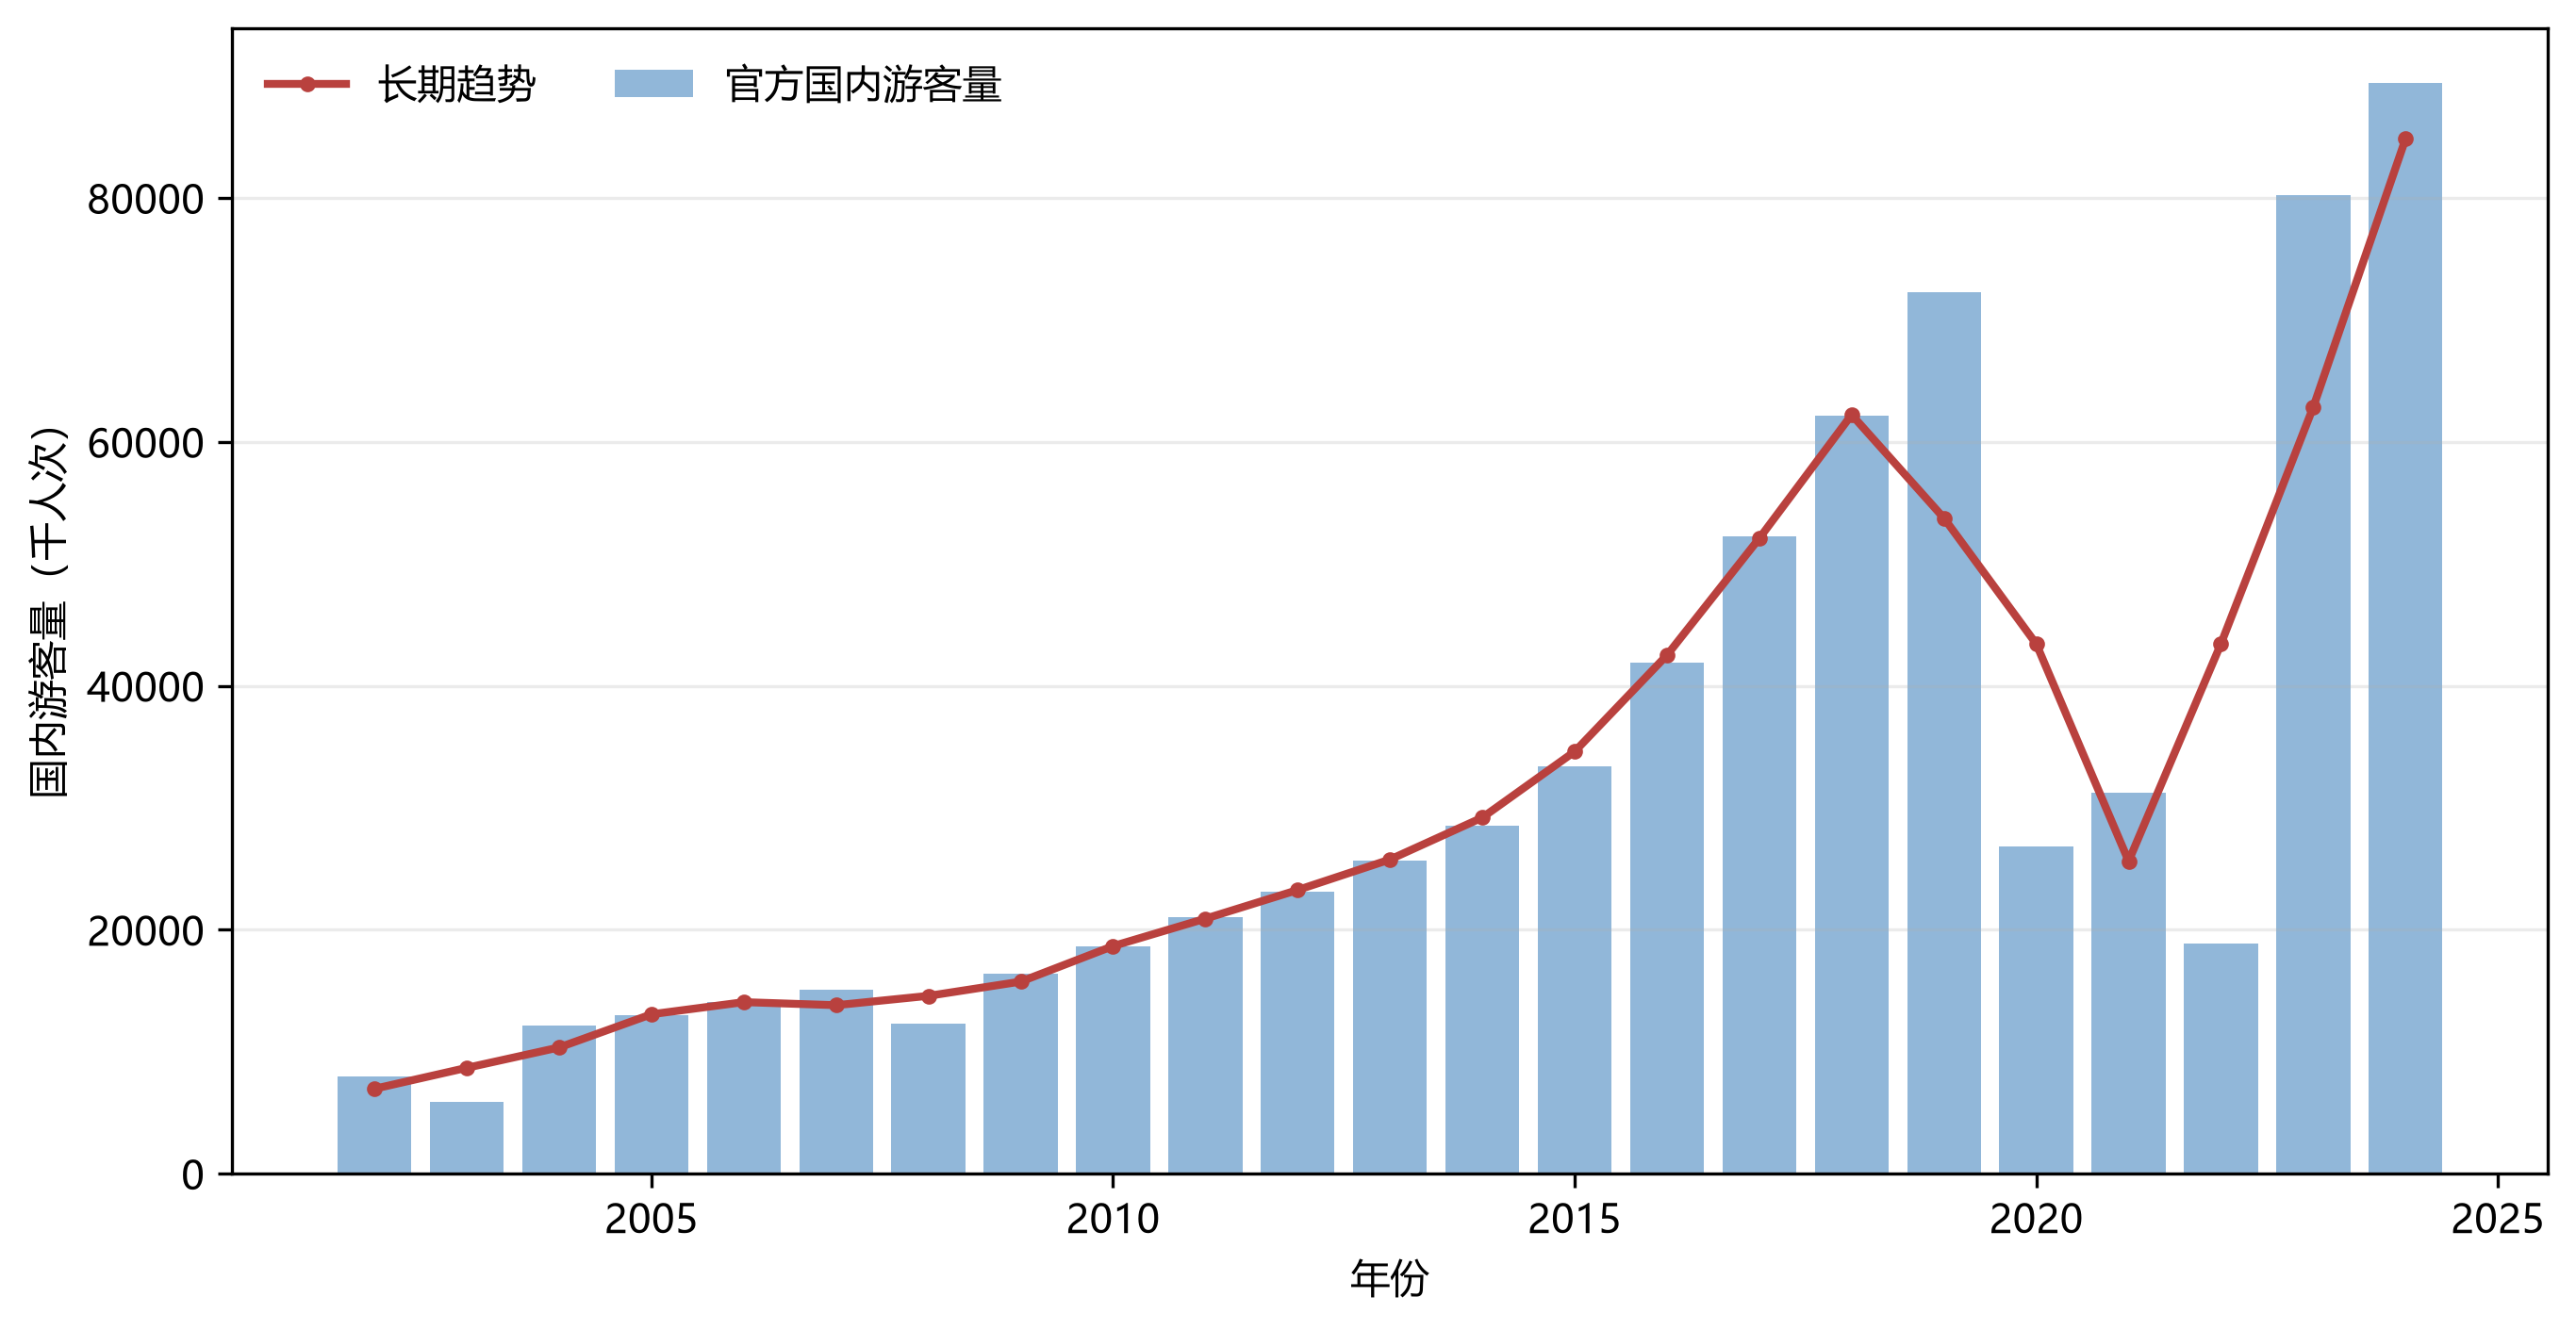
\includegraphics[width=0.93\textwidth]{q1_city_annual_trend.png}
\caption{秦皇岛市年度国内游客量及长期趋势}\label{fig:q1-annual}
\end{figure}

图\ref{fig:q1-pressure}显示2025-06-15至2025-10-10的三区日级压力。北戴河在7月与8月的月度压力中位数分别为0.639和0.606，均被识别为片区旺季；海港--阿那亚的压力基准相对较高；山海关在暑期和国庆窗口出现相对抬升。由于三个指数不具备共同的绝对人数标定，图\ref{fig:q1-pressure}用于识别各片区的时间峰谷和冲击窗口，不用于比较三区真实游客规模。

\begin{figure}[H]\centering
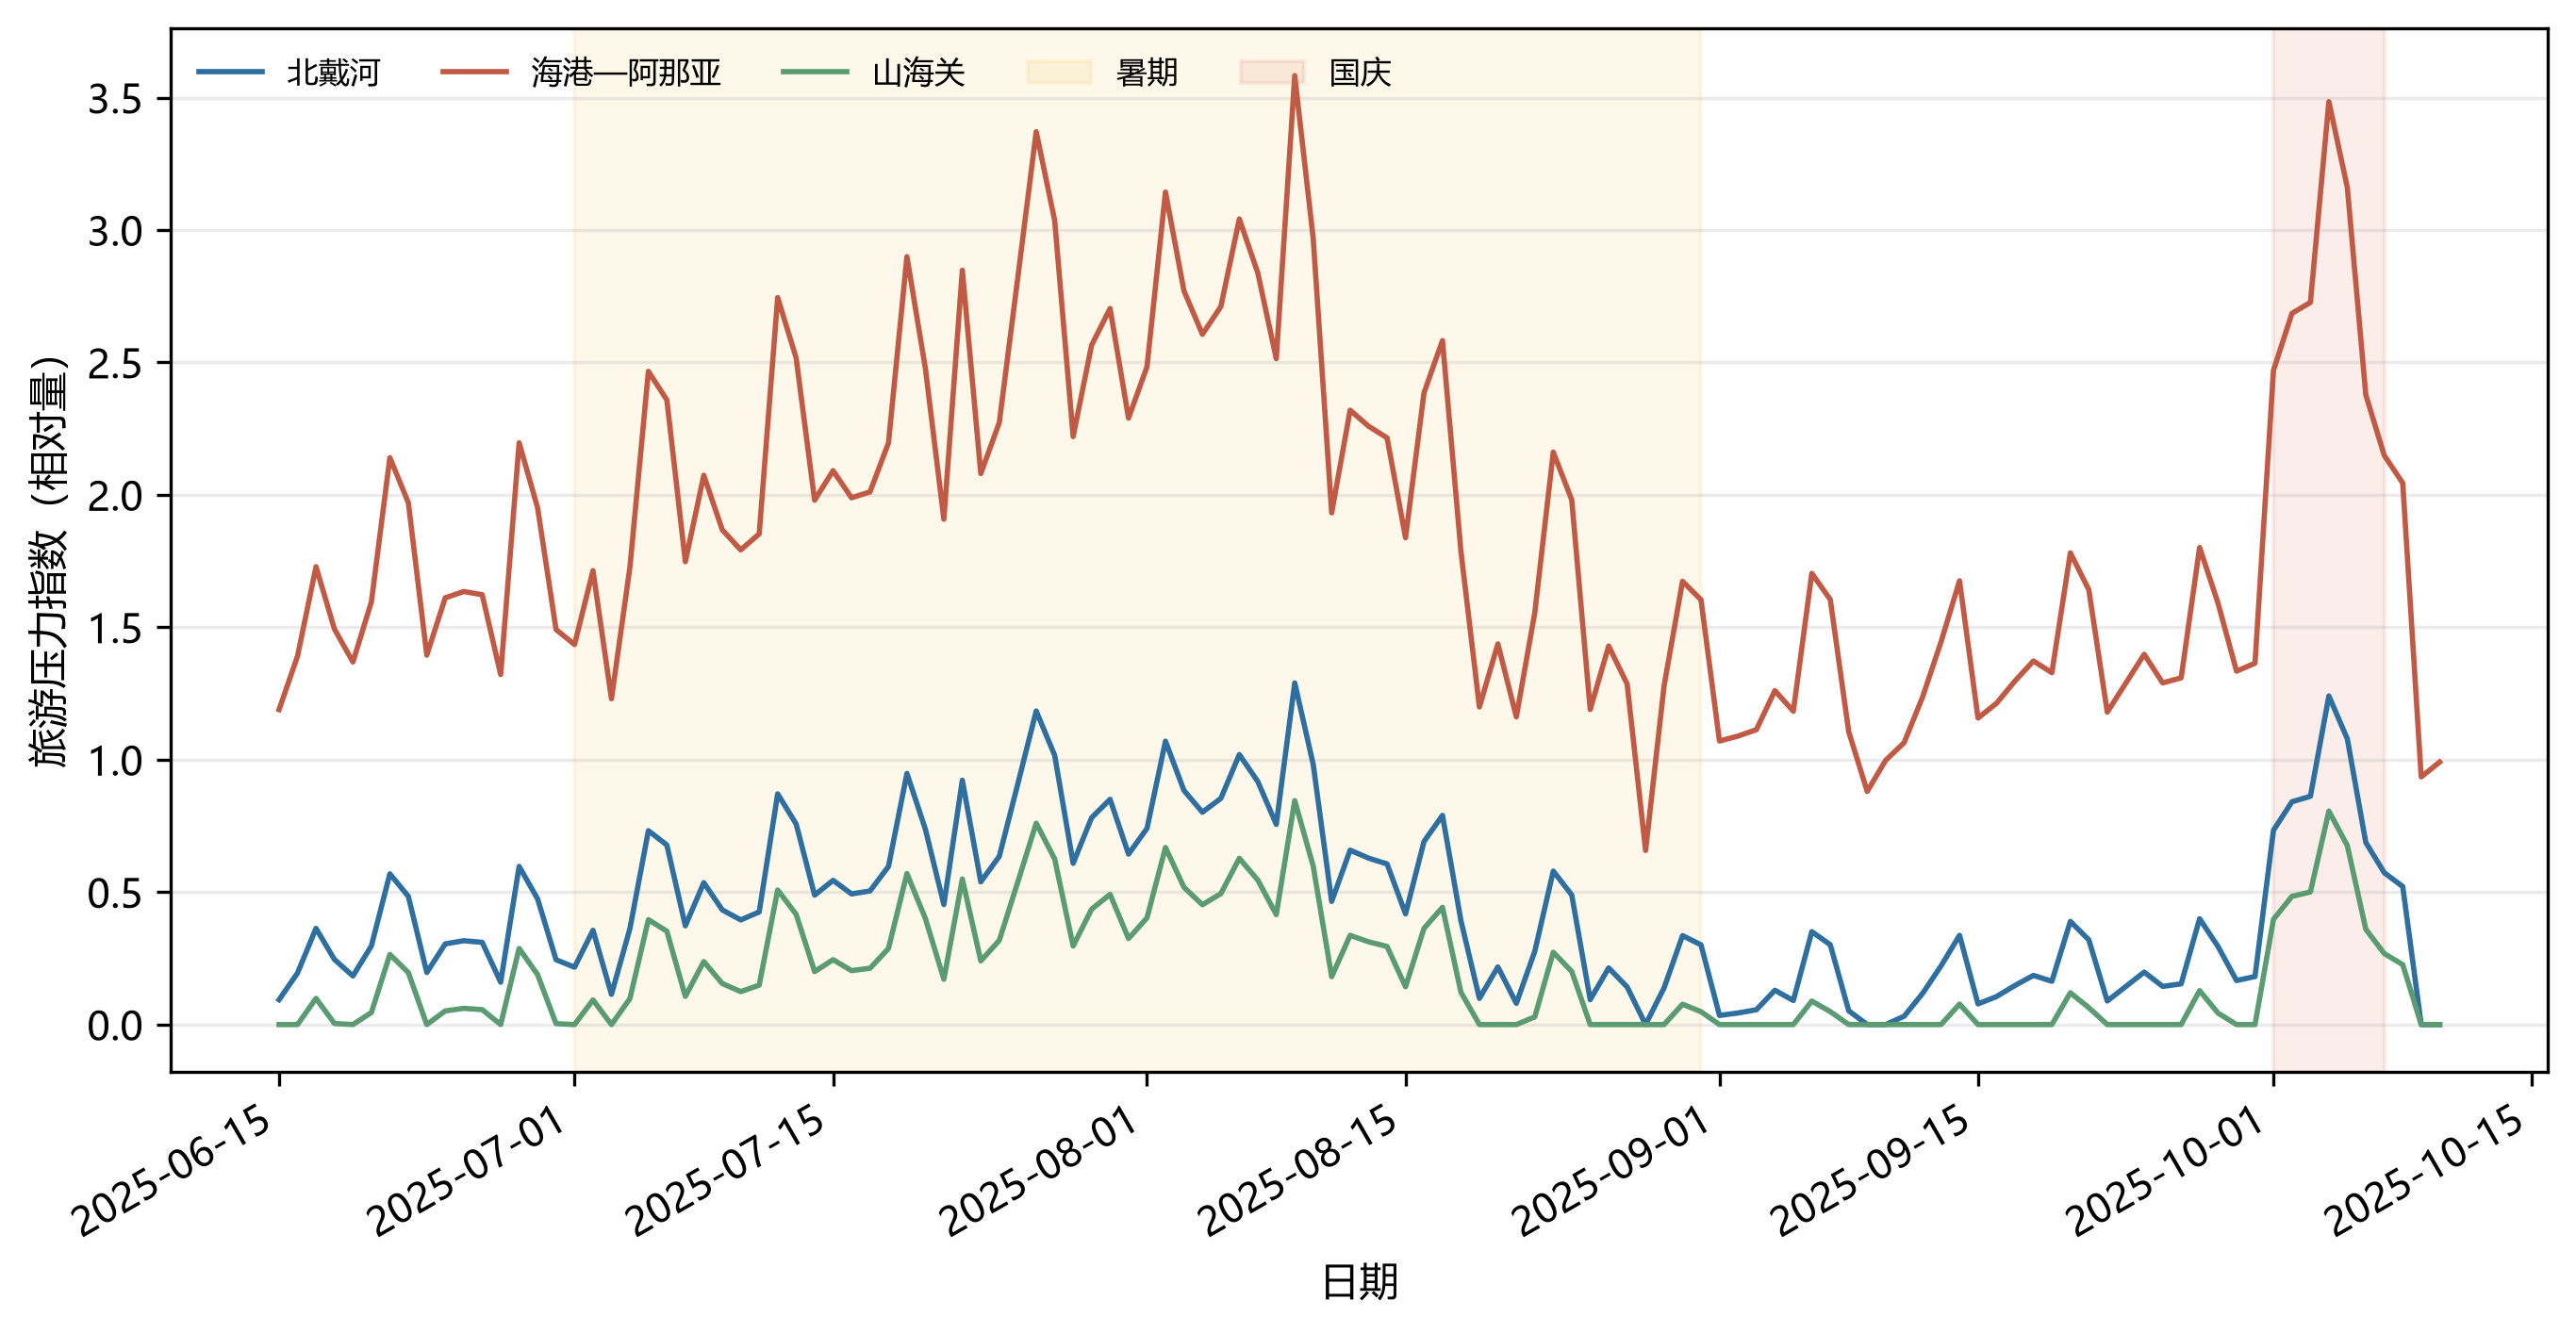
\includegraphics[width=0.93\textwidth]{q1_regional_peak_pressure_2025.png}
\caption{三大片区旺季日级旅游压力（相对量）}\label{fig:q1-pressure}
\end{figure}

以标准化系数的绝对值衡量，滞后一期目的地搜索热度的关联强度为0.244，居各协变量首位；法定节假日与周末的关联强度分别为0.095和0.094；降水的系数为$-0.044$。这些结果只表示模型条件关联，不能作因果解释。

\begin{table}[H]\centering
\caption{主要变量及其模型角色}\label{tab:q1-var}
\begin{tabular}{lll}\toprule
符号&定义&作用与口径\\\midrule
$Y_y$&全市年度国内游客量&年度尺度绝对约束\\
$F_{r,t}$&片区日级旅游压力&相对量，不等同真实日游客数\\
$\mathbf X_t$&搜索、天气、节假日等协变量&解释短期波动\\
$S_t$&隐状态（常态/旺季/冲击）&刻画状态切换\\\bottomrule
\end{tabular}\end{table}

\section{可靠性说明与本问结论}
本问的可验证部分是：全市年度输出受官方年度总量约束；片区序列连续覆盖2023--2025年，并显式保留相对压力口径；日内服务结构仅作为归一化服务时段情景，不被称为实测小时客流。由此可知，秦皇岛全市旅游需求具有长期恢复趋势，三区共同具有暑期和节假日脉冲，但片区基准与峰谷形态不同。问题二以$\widehat Y_t$的年度尺度和$F_{r,t}$的日级形状开展预测；问题三、四只在透明情景参数下使用由预测结果换算的资源需求。

\end{document}
